\clearpage
\section[Fully-coupled model]{Solving a problem using a Fully-Coupled Model}\label{tutorial-coupled}

The process of solving a problem using \Dumux can be roughly divided into four parts:
\begin{enumerate}
 \item The geometry of the problem and correspondingly a grid have to be defined.
 \item Material properties and constitutive relationships have to be defined.
 \item Boundary conditions as well as initial conditions have to be defined.
 \item A suitable model has to be chosen.
\end{enumerate}

The problem that is solved in this tutorial is illustrated in figure \ref{tutorial-coupled:problemfigure}. A rectangular domain with no flow boundaries on the top and on the bottom, which is initially saturated with oil, is considered. Water infiltrates from the left side into the domain. Gravity effects as well as capillarity effects are neglected.

\begin{figure}[h]
\psfrag{x}{x}
\psfrag{y}{y}
\psfrag{no flow}{no flow}
\psfrag{water}{\textbf{water}}
\psfrag{oil}{\textcolor{white}{\textbf{oil}}}
\psfrag{p_w = 2 x 10^5 [Pa]}{$p_w = 2 \times 10^5$ [Pa]}
\psfrag{p_w_initial = 2 x 10^5 [Pa]}{\textcolor{white}{\textbf{$\mathbf{p_{w_{initial}} = 2 \times 10^5}$ [Pa]}}}
\psfrag{S_n = 0}{$S_n = 0$}
\psfrag{S_n_initial = 0}{\textcolor{white}{$\mathbf{S_{n_{initial}} = 0}$}}
\psfrag{q_w = 0 [kg/m^2s]}{$q_w = 0$ $\left[\frac{\textnormal{kg}}{\textnormal{m}^2 \textnormal{s}}\right]$}
\psfrag{q_n = -3 x 10^-4 [kg/m^2s]}{$q_w = -3 \times 10^-4$ $\left[\frac{\textnormal{kg}}{\textnormal{m}^2 \textnormal{s}}\right]$}
\centering
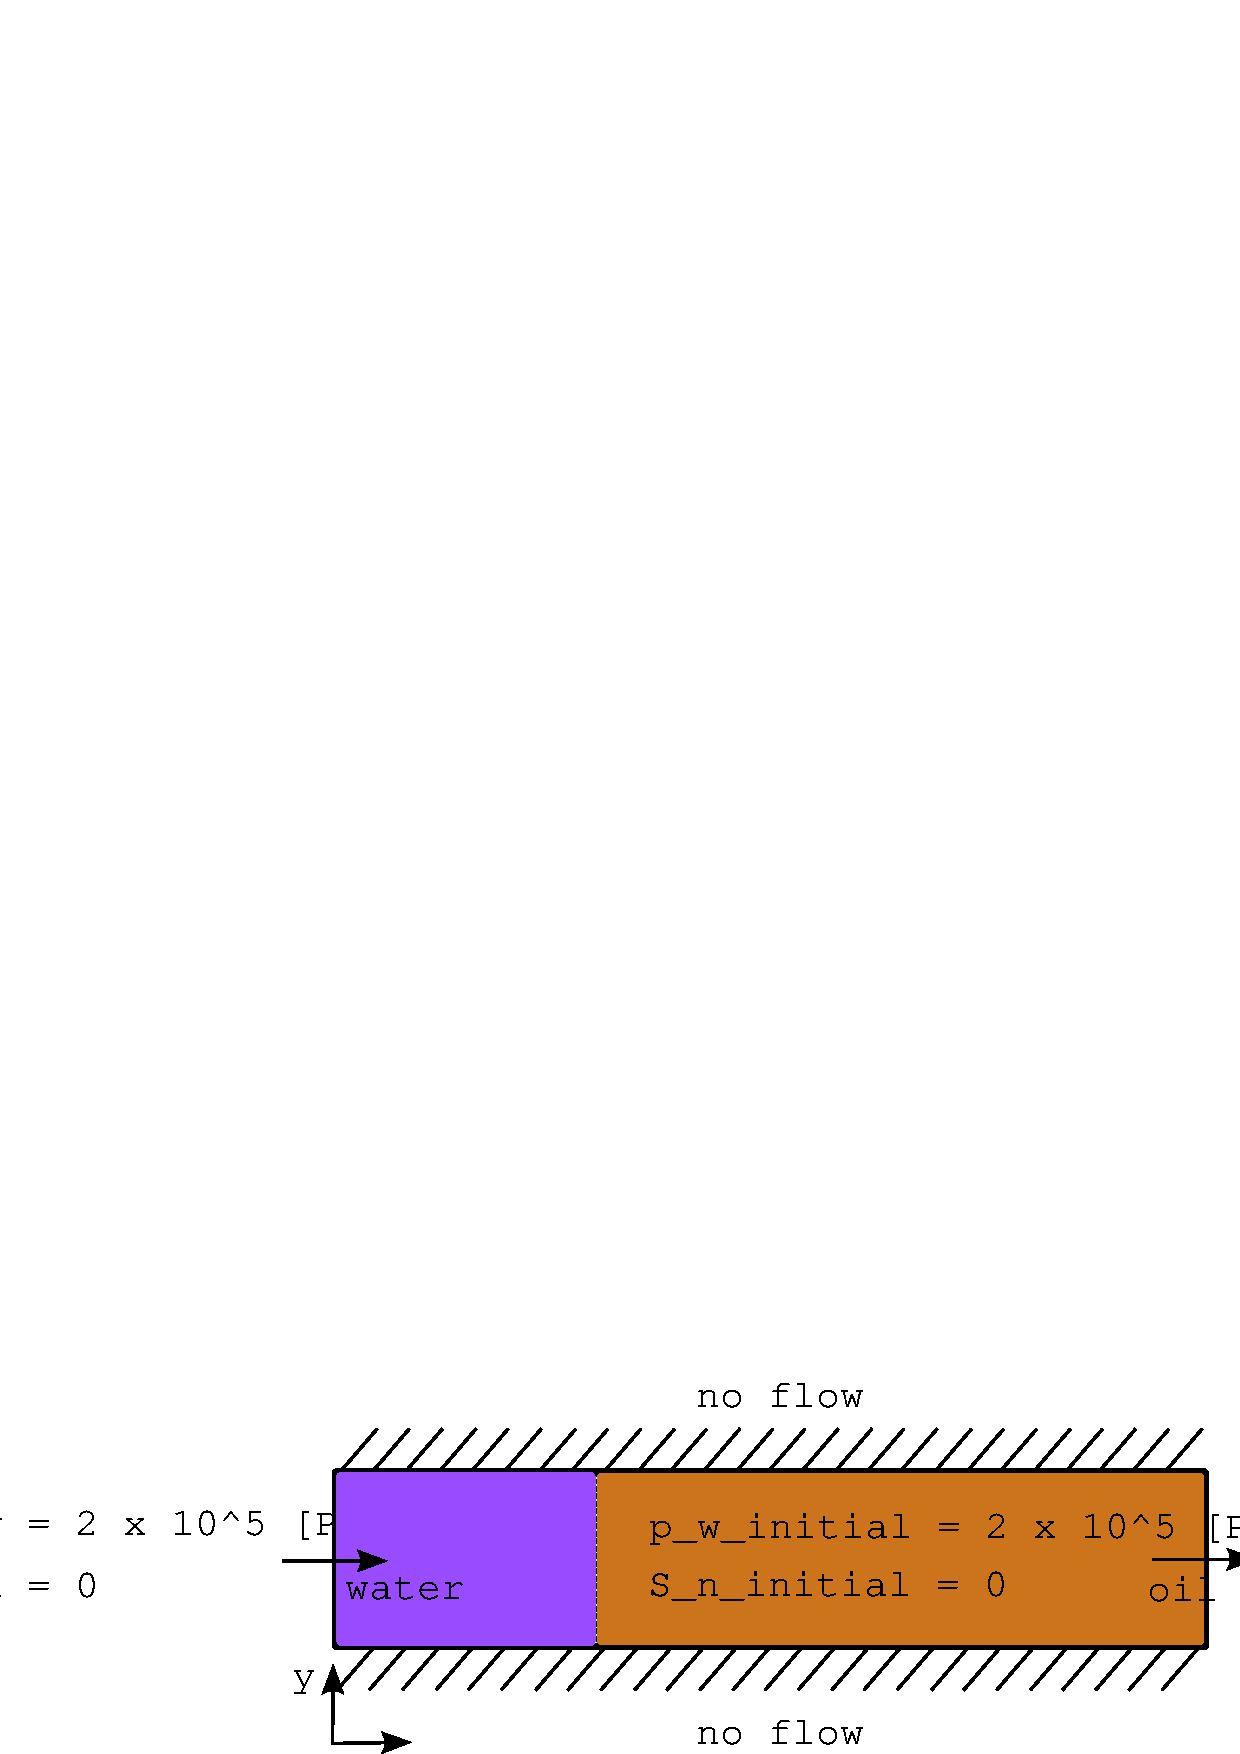
\includegraphics[width=0.9\linewidth,keepaspectratio]{EPS/tutorial-problemconfiguration}
\caption{Geometry of the tutorial problem with initial and boundary conditions.}\label{tutorial-coupled:problemfigure}
\end{figure}

Listing \ref{tutorial-coupled:mainfile} shows the main file \texttt{tutorial\_coupled.cc} for the coupled twophase model. This file needs to be executed to solve the problem described above. The main file can be found in the directory \texttt{/dune-mux/test/tutorial}.

\begin{lst}[File dune-mux/test/tutorial/tutorial\_coupled.cc]\label{tutorial-coupled:mainfile} \mbox{}
\lstinputlisting[basicstyle=\ttfamily\scriptsize,numbers=left,
numberstyle=\tiny, numbersep=5pt]{../../test/tutorial/tutorial_coupled.cc}
\end{lst}

From line \ref{tutorial-coupled:include-begin} to line \ref{tutorial-coupled:include-end} the Dune and the \Dumux files which contain the functions and classes that are needed in the main function are included into the main file.

The geometry of the problem and the grid on which the problem is to be solved are defined in the lines \ref{tutorial-coupled:grid-begin} to \ref{tutorial-coupled:grid-end}. The three variables of Type \texttt{Dune::FieldVector} define the lower left corner of the domain (\texttt{L}), the upper right corner of the domain (\texttt{H}) and the number of cells in $x$ and $y$ direction (\texttt{N}). The dimension \texttt{dim} is previously defined in line \ref{tutorial-coupled:dim}. The grid of type \texttt{Dune::SGrid} is then generated in line \ref{tutorial-coupled:grid-end}. For more information about the dune grid interface, the different grid types that are supported and the generation of different grids it is referred to the \textit{Dune Grid Interface HOWTO (http://www.dune-project.org/doc/)}.

The second step needed to solve the problem is the definition of material properties and constitutive relationships. The fluid properties of the two fluid phases considered here are defined in the lines \ref{tutorial-coupled:water} and \ref{tutorial-coupled:oil}. \Dumux provides several fluid classes which can be found in the file \texttt{phaseproperties2p.hh} in the directory \texttt{/dune-mux/dumux}-\texttt{/material/phaseproperties}. \\
The properties of the solid matrix are defined in a special soil class. The \texttt{soil} object is generated in line \ref{tutorial-coupled:soil}. As can be seen, the class type is \texttt{Dune::TutorialSoil}, which is defined in the file \texttt{tutorial\_soilproperties.hh} in the folder \texttt{/test/tutorial}. A description of this file and the definition of a soil class including the soil parameters can be found in section \ref{tutorial-coupled:description-soil-class}. Finally, in line \ref{tutorial-coupled:twophaserelations} the information included in the fluid and soil objects is used to generate an object of type \texttt{Dune::TwoPhaseRelations}, which includes the constitutive relationships (capillary pressure-saturation relation, relative permeability-saturation relation, etc.). The file \texttt{twophaserelations.hh} can be found in the directory \texttt{/dune-mux/dumux/material}.


